\fancyhf{}
\pagestyle{fancy}
%Encabezado
\lhead[]{\leftmark}
\chead[]{}
\rhead[]{\thepage}
\renewcommand{\headrulewidth}{1pt}

\section{Introducción}

En este capítulo, se presentan tres casos de estudio que fueron seleccionados para que sean analizados por Identifier Analyzer (IDA). En cada uno de estos casos se examinan los identificadores (ids) de una aplicación JAVA. A través de tablas se irán mostrando los resultados obtenidos, producto de la ejecución de las técnicas que IDA posee.
Con estos casos, se pretende manifestar la utilidad de la herramienta IDA en lo que respecta al análisis de ids y demostrar que es un aporte al área de la CP. A continuación, se listan las aplicaciones JAVA que serán analizadas por IDA:

\begin{itemize}
\itemsep0em%reduce espacio
\item Juego Buscaminas: Minesweeper
\item Editor de Texto
\item Juego de Aviones: Top Gun
\end{itemize}

En las próximas secciones, se describe el análisis realizado de cada una.

\begin{figure}[h!] %[h] para here [b] para bottom [t] para top
\centerline{%queda centrada mejor la imagen
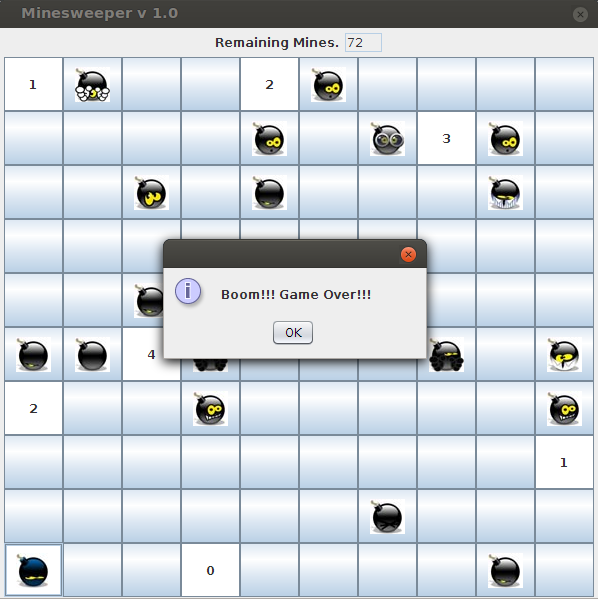
\includegraphics[scale= 0.6]{./cap5/caso_01.png}
}
\caption{Captura del Juego Buscaminas programado en JAVA}
\label{caso1}
\end{figure}

\section{Juego Buscaminas}

El programa JAVA denominado Minesweeper.java, al ejecutarlo posee el clásico y conocido juego llamado Buscaminas (Minesweeper en Inglés - Ver Figura \ref{caso1}). El juego consiste en despejar los casilleros de un tablero que posee minas, estas minas están ocultas y el jugador pierde en caso de detonar alguna.
Este programa contiene un módulo de 250 líneas aproximadamente que fueron analizadas por IDA.

\noindent \textbf{\\Captura de Información\\} 

Al ingresar el programa Minesweeper.java a la herramienta IDA, se da comienzo a la fase de extracción de datos y el analizador sintáctico (AS) captura información referente a los ids. Esta información la exhibe IDA al usuario en el \textit{Panel de Elementos Capturados}, en la tabla \textit{Declaraciones} (Ver Capítulo anterior). En la tabla \ref{tabla2} se puede apreciar esta información (por columnas): la línea donde está declarado el id, el nombre, que representa en el código analizado, el tipo del id y que modificador posee.

Para hacer una descripción más detallada sobre los ids capturados, en la tabla \ref{tabla2} se puede observar que el archivo \mbox{Minesweeper.java}
tiene ids del tipo \textit{hardwords} y \textit{softwords} (Ver Capítulo 3 - sección \ref{sec:clasif}). Algunos \textit{hardwords} que se pueden observar son \textsf{min\_mtrx}, \textsf{TOTmin}, \textsf{topPanel} (entre otros), ya que estos poseen una marca de separación que destacan las palabras que lo componen. Por otro lado, algunos de los \textit{softwords} que se capturaron son \textsf{ae}, \textsf{plantmines}, \textsf{bttns}, \textsf{xar} (entre otros).
A su vez, se capturaron los comentarios, los mismos se muestran en tabla \ref{tabla3}\footnote[1]{Los comentarios de más de una línea (comprendidos entre /* */), se descomponen en líneas diferentes.}. De la misma forma, los literales Strings que se extrajeron se exhiben en la tabla \ref{tabla4}. En ambas tablas se muestran las líneas en donde se ubica cada comentario y literal en el código.
Tanto los literales y los comentarios se visualizan en IDA a través del \textit{Panel de Elementos Capturados}, eligiendo la pestaña correspondiente (Ver Capítulo anterior).

Es importante recordar, que los comentarios y literales de las tablas \ref{tabla3} y \ref{tabla4} son usados para construir la lista de frases que se muestra en la ventana de \textit{Palabras Capturadas} (Ver Capítulo anterior). Esta información es útil para el Algoritmo de Expansión. De la misma manera, con los comentarios y literales se construye una parte importante del listado de frecuencias locales de aparición de palabras\footnote[2]{En este contexto, se refiere a palabras que están contenidas en literales, comentarios e ids, este último necesita un proceso especial, para más detalles ver Cap. 3 - sección \ref{sec:algSamu}}, que son destinadas a ser usadas por el Algoritmo de división Samurai. Esta lista se visualiza en IDA también dentro de la ventana de \textit{Palabras Capturadas} (Ver Capítulo anterior).\\

Habiendo explicado con este caso de estudio la información capturada por el AS, asociada a ids, literales y comentarios, en la próxima sección se procede a analizar (para este mismo caso de estudio), los resultados obtenidos producto del análisis de los ids. 

\begin{sidewaystable}[h!]
\centering
	\begin{tabular}{| c | c | c | c | c |}      
       \hline
  	   \textbf{Línea} & \textbf{Nombre ID} & \textbf{Representa} & \textbf{Tipo} & \textbf{Modificador} \\ \hline
7&Minesweeper&Clase&--&public \\ \hline
10&bttns&Variable de Clase&JButton&private \\ \hline
12&min\_mtrx&Variable de Clase&int&private \\ \hline
14&txtMin&Variable de Clase&JTextField&private \\ \hline
17&rm&Variable de Clase&JLabel&private \\ \hline
20&min\_imag&Variable de Clase&ImageIcon&private \\ \hline
22&dim&Variable de Clase&int&private \\ \hline
24&TOTmin&Variable de Clase&int&private \\ \hline
25&sq&Variable de Clase&int&private \\ \hline
%28&Minesweeper&Constructor&--&public \\ \hline
37&topPanel&Variable Local&JPanel&-- \\ \hline
48&middlePanel&Variable Local&JPanel&-- \\ \hline
71&plantmines&Método de Clase&void&private \\ \hline
71&mins&Parámetro&int&-- \\ \hline
102&main&Método de Clase&void&public \\ \hline
102&args&Parámetro&String[]&-- \\ \hline
107&actionPerformed&Método de Clase&void&public \\ \hline
107&ae&Parámetro&ActionEvent&-- \\ \hline
124&uncoverEmpty&Método de Clase&void&private \\ \hline
124&j&Parámetro&int&-- \\ \hline
124&i&Parámetro&int&-- \\ \hline
%134&restart&Método de Clase&void&private \\ \hline
150&win&Método de Clase&void&private \\ \hline
159&boom&Método de Clase&void&private \\ \hline
172&msgDialog&Variable Local&String&-- \\ \hline
179&nearbyMines&Método de Clase&int&private \\ \hline
188&MINSnum&Variable Local&int&-- \\ \hline
179&xar&Parámetro&int&-- \\ \hline
179&yac&Parámetro&int&-- \\ \hline
   
   	\end{tabular}  
	 
   \caption{Identificadores extraídos por el AS ANTLR}
   \label{tabla2}
     
\end{sidewaystable} 


\begin{table}[ht!]
\parbox{.40\linewidth}{
 
		\centering
   		\begin{tabular}{| c | c |}  
       \hline
\textbf{Línea} & \textbf{Comentario} \\ \hline
9&buttons  \\ \hline
13&Text Fields  \\ \hline
16&Labels  \\ \hline
19&Mines images  \\ \hline
21&Dimension  \\ \hline
23&total mines  \\ \hline
27&Time tp  \\ \hline
31&load Images  \\ \hline
36&Top Panel  \\ \hline
47&Button panel  \\ \hline
50&Create and place button  \\ \hline
53&Create Button  \\ \hline
55&Place button  \\ \hline
57&Action Listener  \\ \hline
63&Window properties  \\ \hline
80&Legend of mines in Matrix  \\ \hline
81&1 contains Mine  \\ \hline
82&0 Not contains Mine  \\ \hline
83&Place random mine  \\ \hline
\end{tabular}
}
\hfill
\parbox{.48\linewidth}{
 
		\centering
   		\begin{tabular}{| c | c |}  
       \hline
\textbf{Línea} & \textbf{Comentario} \\ \hline
85&Generate random position \\ \hline
91&Place mine \\ \hline
93&Display mines panel \\ \hline
107&Action Event \\ \hline
126&Uncover an empty square \\ \hline
129&Nearby Mines \\ \hline
136&restart game \\ \hline
152&Win the game \\ \hline
161&lose the game \\ \hline
165&Mines Random Images \\ \hline
183&x axe row \\ \hline
184&y axe column \\ \hline
186&return the number of mines \\ \hline
192&horizontal \\ \hline
199&vertical \\ \hline
207&diagonal \\ \hline
208&Top left corner \\ \hline
209&copy of axes \\ \hline
224&top right corner \\ \hline
\end{tabular}
}
\caption{Comentarios extraídos por el AS ANTLR}\label{tabla3}
\end{table}


\begin{table}[h!]
	
		\centering
   		\begin{tabular}{| c | c |}      
       \hline
  	   \textbf{Línea} & \textbf{Literal} \\ \hline
17&“Remaining Mines.” \\ \hline
33&“.jpg”  \\ \hline
42&“North”  \\ \hline
61&“Center”  \\ \hline
65&“Minesweeper v 1.0 ”  \\ \hline
73&“Planting Mines...”  \\ \hline
153&“You Win!!! Game Over!!!” \\ \hline
155&“Message” \\ \hline
173&“Boom!!! Game Over!!!” \\ \hline
175&“Message” \\ \hline
  \end{tabular} 
	 
   \caption{Literales extraídos por el AS ANTLR}
   \label{tabla4}
     
\end{table} 

\clearpage

\noindent \textbf{Análisis de Resultados\\}

Cuando el usuario ejecuta las técnicas de análisis de ids, lo lleva a cabo mediante la \textit{Ventana de Análisis} (Ver Capítulo anterior), aquí se aplican las técnicas de división (Greedy y Samurai) y después la técnica de expansión de abreviaturas. Esta misma ventana, muestra debajo los resultados obtenidos, luego de ejecutar las técnicas. Para el caso del programa Minesweeper.java, los resultados que se obtuvieron producto del análisis de ids, se pueden apreciar en la Tabla \ref{tabla5}.

Con respecto a la información mostrada en la tabla mencionada previamente, las columnas de \textit{Greedy} y \textit{Samurai} muestran los resultados de división de dichos Algoritmos. En las columnas \textit{Expansión desde Greedy} y \textit{Expansión desde Samurai} se enumeran las expansiones realizadas de las distintas partes del id, que fueron efectuadas desde los Algoritmos Greedy y Samurai respectivamente.

Los ids analizados por IDA de Minesweeper.java (Ver Tabla \ref{tabla5}), en lo que respecta a \textit{hardwords}, se pueden encontrar con guión bajo: \textsf{min\_imag}, \textsf{min\_mtrx} para el tipo camel-case:  \textsf{uncoverEmpty}, \mbox{\textsf{msgDialog}} y para el caso especial: \textsf{TOTmin}, \textsf{MINSnum} (variante camel-case), entre otros. 

El algoritmo Greedy manifiesta irregularidades a la hora de dividir ya que siempre considera que la mayor cantidad de divisiones es la mejor opción (Ver Capítulo 3 - sección \ref{sec:algGre}), esto puede observarse en casos como \textsf{min--im--ag},  \textsf{bt--tn--s}, \textsf{min--sn--um} (Ver Tabla \ref{tabla5} - columna Greedy).
Para los ids que son del tipo especial: \textsf{MINSnum}, \textsf{TOTmin} (variante camel-case), es interesante observar como Samurai realiza la división correctamente: \textsf{mins--num}, \textsf{tot--min} (Ver Capítulo 3 - sección \ref{sec:algSamu}), y no la considera un caso común de camel-case que la separa antes de la mayúscula seguido de minúscula. Esto sucede justamente con Greedy ya supone que es del tipo camel-case, y realiza la separación incorrecta: \mbox{\textsf{min--sn--um}} (entre min y sn), \textsf{to--tm--in} (entre to y tm).

En lo que respecta a \textit{softwords} se aprecia la presencia de acrónimos como \textsf{rm} y \textsf{ae} (entre otros); ambos algoritmos de división no los dividen. La razón de esto es porque  poseen solo dos caracteres y el algoritmo lo considera acrónimos.
 A la hora de expandir \textsf{rm}, \textsf{ae}, el Algoritmo de Expansión consulta la lista de frases conformada en su mayoría por los comentarios y literales capturados (Ver Tablas \ref{tabla3} y \ref{tabla2}), al encontrar coincidencia con el literal \textsf{“remaining mines”} y el comentario \textsf{action event}, selecciona ambos como la expansión correspondiente de \textsf{rm} y \textsf{ae} (Ver Tabla \ref{tabla5} - Columnas de Expansión).
El resto de los softwords se puede considerar a \textsf{mins}, \textsf{bttns}, \textsf{dim}, aquí Greedy también acusa inconvenientes y procede a separar estos ids siendo que no se deben separar, caso contrario ocurre con Samurai (Ver Tabla \ref{tabla5} - Columnas de División). %falta mostrar las tablas de frecuencias

Continuado en la tabla \ref{tabla5}, los ids \textsf{i}, \textsf{j} son comunes en la mayoría de los códigos, y generalmente se utilizan como contadores en estructuras de control iterativas (\textsf{for}, \textsf{while}, etc). En estos casos, el Algoritmo de Expansión busca palabras que estén dentro del \textit{Dominio del Problema}. Para lograrlo, recurre a las tablas de Literales y Comentarios (Ver Tablas \ref{tabla3} y \ref{tabla4}), luego trata de encontrar palabras que comiencen con las letras respectivas, para este caso \textsf{image}, \textsf{jpg}. De esta manera el algoritmo, trata de darle una traducción válida en este contexto. En caso de no haber coincidencia con ninguna, el algoritmo de expansión buscará en el diccionario de palabras en Inglés.

Para concluir, en las columnas de expansión de la tabla \ref{tabla5} se visualizan palabras como: ventana, vacío, plantar, minas, recuadro, botones, panel (entre otras). Estas palabras intuitivamente se consideran que forman parte del \textit{Dominio del Problema} correspondiente al programa Minesweeper.java.


\begin{sidewaystable}[h!]

		\centering
   		\begin{tabular}{| c | c | c | c | c |}     
   		
       \hline
  	   \textbf{Id} & \textbf{Greedy} & \textbf{Samurai} & \textbf{Exp. desde Greedy} & \textbf{Exp. desde Samurai} \\ \hline
Minesweeper&minesweeper&minesweeper&minesweeper&minesweeper\\ \hline
bttns&bt--tn--s&bttns&button tn square&buttons\\ \hline
min\_mtrx&min--mt--rx&min--mtrx&mines matrix rx&mines matrix\\ \hline
txtMin&txt--min&txt--min&text mines&text mines\\ \hline
rm&rm&rm&remaining mines&remaining mines\\ \hline
min\_imag&min--im--ag&min--imag&mines images ag&mines images\\ \hline
dim&dim&dim&dimension&dimension\\ \hline
TOTmin&to--tm--in&tot--min&to total mines in&total mines\\ \hline
sq&sq&sq&square&square\\ \hline
%Minesweeper&minesweeper&minesweeper&minesweeper&minesweeper\\ \hline
topPanel&top--panel&top--panel&top panel&top panel\\ \hline
middlePanel&middle--panel&middle--panel&middle panel&middle panel\\ \hline
plantmines&plant--mines&plant--mines&planting minesweeper&planting minesweeper\\ \hline
mins&min--s&mins&mines square&mines\\ \hline
%main&main&main&main&main\\ \hline
%args&args&args&args&args\\ \hline
actionPerformed&action--performed&action--performed&action performed&action performed\\ \hline
ae&ae&ae&action event&action event\\ \hline
uncoverEmpty&uncover--empty&uncover--empty&uncover empty&uncover empty\\ \hline
j&j&j&jpg&jpg\\ \hline
i&i&i&images&images\\ \hline
%restart&restart&restart&restart&restart\\ \hline
win&win&win&window&window\\ \hline
%msgDialog&msg--dialog&msg--dialog&message dialog&message dialog\\ \hline
boom&boom&boom&boom&boom\\ \hline
msgDialog&msg--dialog&msg--dialog&message dialog&message dialog\\ \hline
nearbyMines&nearby--mines&nearby--mines&nearby minesweeper&nearby minesweeper\\ \hline
%yac\_cp&y--ac--cp&yac--cp&year action copy&y axe column copy\\ \hline
%xar\_cp&xa--r--cp&xar--cp&xa row copy&x axe row copy\\ \hline
MINSnum&min--sn--um&mins--num&mines sn um&mines number\\ \hline
xar&xa--r&xar&xa row&x axe row\\ \hline
yac&y--ac&yac&yellow action&y axe column\\ \hline

  \end{tabular}
	 
   \caption{Análisis Realizado a los Ids extraídos de Minesweeper.java}
   \label{tabla5}
     
\end{sidewaystable}

\clearpage %esto es necesario sino las tablas se van al final del capitulo

\begin{figure}[t] %[h] para here [b] para bottom [t] para top
\centerline{%queda centrada mejor la imagen
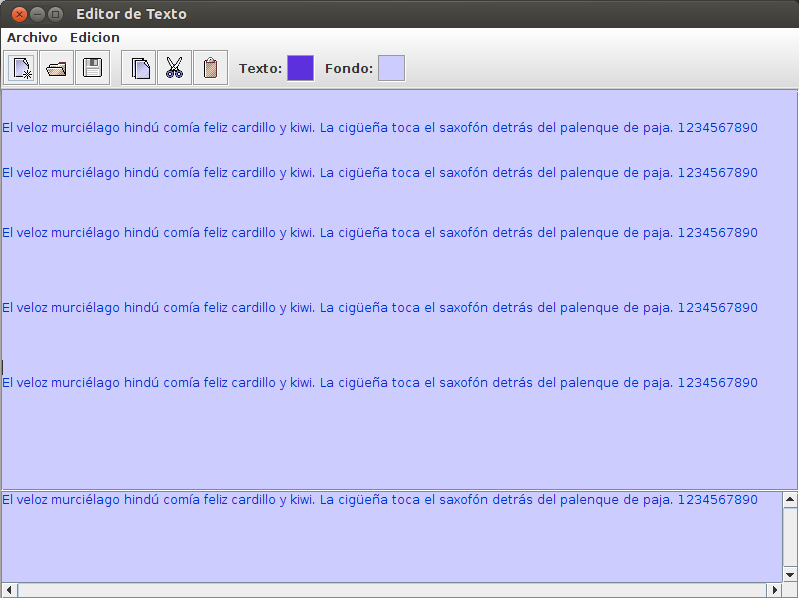
\includegraphics[scale= 0.64]{./cap5/caso_02.png}
}
\caption{Captura del Editor de Texto programado en JAVA}
\label{caso2}
\end{figure}

\section{Editor de Texto}

En el próximo caso de estudio, se seleccionó un programa escrito en JAVA que corresponde a un editor de texto (Ver Figura \ref{caso2}). Este editor posee las herramientas básicas para crear o modificar archivos de textos sin formato, permite cambiar la visualización de colores en las letras y en el fondo, también imprime los archivos que se abran en el.
Este editor esta programado con alrededor de 500 líneas de código, las cuales están escritas en un único archivo llamado Editor.java. 

Cabe destacar que, a modo de facilitar la lectura, de aquí en adelante, por cada caso de estudio, se mostrará únicamente la tabla con resultados obtenidos producto del análisis de los ids y se excluirán el resto de las tablas que se mostraron en el caso de estudio anterior. El proceso es el mismo y por lo tanto no tiene sentido volverlo a escribir.

A continuación, se brindan los resultados obtenidos de analizar con la herramienta IDA el editor de textos, el análisis efectuado en los ids se exhibe en la tabla \ref{tabla6}. Dado que este programa posee muchos ids, los resultados que se presentan en la tabla \ref{tabla6} son los más destacados y no son la totalidad.\\

\noindent \textbf{Análisis de Resultados\\}

A simple vista, se puede observar en la tabla \ref{tabla6}, que nuevamente las divisiones de Samurai son las que mejor se realizan.
Como se explicó anteriormente, esto ocurre por que Greedy siempre selecciona la mayor cantidad de divisiones en la palabra como la mejor opción (Ver Capítulo 3 - sección \ref{sec:algGre}). Algunos ejemplos de divisiones mal hechas por Greedy son \textsf{bckCol} $\rightarrow$ \textsf{b--c--k--col},
\textsf{btAcept} $\rightarrow$ \textsf{bt--ace--pt}, \textsf{jChoColor} $\rightarrow$ \textsf{j--c--ho--color}, entre otros. 

Sin embargo, en este caso de estudio a diferencia del anterior existen algunas divisiones en las que Samurai falla, los ids que se pueden observar son: \textsf{flreader}, \textsf{ptjob} los cuales directamente no se dividieron como lo hizo Greedy en \mbox{\textsf{fl--reader}}, \textsf{pt--job}. La primer hipótesis que se maneja sobre este resultado, es que Greedy encuentra en el diccionario en Inglés las palabras \textsf{reader} y \textsf{job} y con esto basta para llevar a cabo la división. Mientras que Samurai en su función de \textit{Score}, las palabras \textsf{fl} con \textsf{reader} y \textsf{pt} con \textsf{job} no representan puntajes (score) altos para ser divididas entre ellas (Ver Capítulo 3 - sección \ref{sec:algSamu}). En este caso de estudio, al igual que el anterior, también existen casos de variante de camel-case, algunos son:\textsf{TEXTarea}, \textsf{PRGname} y el algoritmo Samurai los divide correctamente, mientras que Greedy no (Ver Tabla \ref{tabla6}).

En lo que respecta a la expansión de ids, la mayoría de las abreviaturas resultantes de la división de ids fueron expandidas; algunos ejemplos son \textsf{sel} $\rightarrow$ \textsf{select}, \textsf{tl} $\rightarrow$ \textsf{tool}, \textsf{cl} $\rightarrow$ \textsf{close}, \textsf{bck} $\rightarrow$ \textsf{background}, entre otras. Estas palabras son expandidas por el algoritmo de expansión, gracias a los comentarios y literales capturados por el AS.
Por otro lado, existen algunas abreviaturas que no se expanden como es el caso de \textsf{bt} a \textsf{button}, \textsf{it} a \textsf{item}; que forman parte de los ids \textsf{bt--acept} y \textsf{men--it--new}. La hipótesis de este comportamiento en el Algoritmo de Expansión, se debe a que estas abreviaturas son tratadas como acrónimos (abreviaturas con más de una palabra) dado que tienen solo dos caracteres y no existe una frase (de comentarios o literales) capturada por el AS, que coincida. Como se consideran abreviaturas con más de una palabra, tampoco se utiliza el diccionario en Inglés para expandir.


\begin{sidewaystable}[h!]

		\centering
   		\begin{tabular}{| c | c | c | c | c |}     
   		
       \hline
  	   \textbf{Id} & \textbf{Greedy} & \textbf{Samurai} & \textbf{Exp. desde Greedy} & \textbf{Exp. desde Samurai} \\ \hline

%jMenBar&j--men--bar&j--men--bar&java menu background&java menu background\\ \hline
menBarFile&men--bar--file&men--bar--file&menu background file&menu background file\\ \hline
menItNew&men--it--new&men--it--new&menu it new&menu it new\\ \hline
menBarEdit&men--bar--edit&men--bar--edit&menu background editor&menu background editor\\ \hline
menItCopy&men--it--copy&men--it--copy&menu it copy&menu it copy\\ \hline
jTlBar&j--tl--bar&j--tl--bar&java tool background&java tool background\\ \hline
jBtSave&j--bt--save&j--bt--save&java bt save&java bt save\\ \hline
popUpMenu&pop--up--menu&pop--up--menu&pop up menu&pop up menu\\ \hline
imIcPrint&im--ic--print&im--ic--print&images icon printing&images icon printing\\ \hline
PRGname&pr--g--name&prg--name&program gif name&program name\\ \hline
jLabelColTex&j--label--col--t--ex&j--label--col--tex&java label color text exit&java label color text\\ \hline
bckCol&b--c--k--col&bck--col&bar copy kilo color&background color\\ \hline
TEXTarea&t--ex--tare--a&text--area&text exit tare areas&text areas\\ \hline
textAREAerrors&t--ex--tare--ae--rrors&text--area--errors&text exit tare areas rrors&text areas errors\\ \hline
jScrPANtxtAr&j--scr--pa--nt--xt--ar&j--scr--pan--txt--ar&\shortstack{java scrollbar program\\north xt areas}&\shortstack{java scrollbar\\pan text areas} \\ \hline
selCl&sel--c--l&sel--cl&select copy literalizes&select close\\ \hline
fc&f--c&fc&finish copy&fc\\ \hline
flreader&fl--reader&flreader&file reader&flreader\\ \hline
ioe&io--e&ioe&icon editor&invoiced\\ \hline
printText&print--text&print--text&printing text&printing text\\ \hline
ptjob&pt--job&ptjob&printing job&ptjob\\ \hline
pg&pg&pg&print graphics&print graphics\\ \hline
%init&init&init&init&init\\ \hline
linNum&l--in--nu--m&lin--num&lab in nu menu&linearised numerically\\ \hline
i&i&i&images&images\\ \hline
jLbFind&j--lb--find&j--lb--find&java lb find&java lb find\\ \hline
jTxFind&j--tx--find&j--tx--find&java text find&java text find\\ \hline
%ed&ed&ed&editor&editor\\ \hline
jPanBut&j--pan--but&j--pan--but&java pan but&java pan but\\ \hline
%jTxWord&j--tx--word&j--tx--word&java text word&java text word\\ \hline
jChoColor&j--c--ho--color&j--cho--color&java copy ho color&java choose color\\ \hline
btAcept&bt--ace--pt&bt--acept&bt ace printing&bt acept\\ \hline

  \end{tabular}
	 
   \caption{Parte del Análisis Realizado a los Ids de Editor.java}
   \label{tabla6}
     
\end{sidewaystable}

\clearpage %esto es necesario sino las tablas se van al final del capitulo

\begin{figure}[h!] %[h] para here [b] para bottom [t] para top
\centerline{%queda centrada mejor la imagen
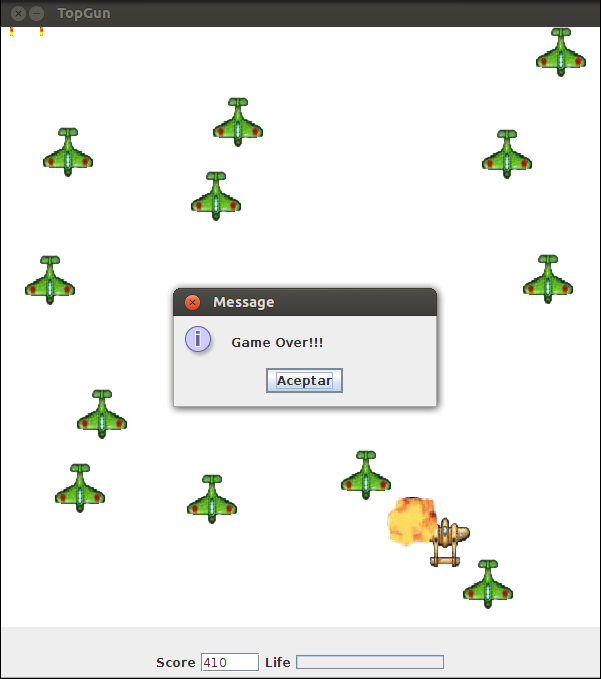
\includegraphics[scale= 0.72]{./cap5/caso_03.png}
}
\caption{Captura del juego Top Gun programado en JAVA}
\label{caso3}
\end{figure}

También existen casos de abreviaturas mal expandidas, uno de ellos es \textsf{bar} $\rightarrow$ \textsf{background}. Si bien \textsf{bar} hace referencia a “barra” en el id \textsf{menBarEdit}, aquí simplemente el algoritmo de expansión entiende que \textsf{bar} es una abreviatura y la expande con un candidato fuerte que se encuentra en el listado de frases capturadas \textsf{\textbf{ba}ckg\textbf{r}ound}.

La mayoría de los ids analizados (Ver Tabla \ref{tabla6} columnas Expansión desde Greedy y Expansión desde Samurai), se corresponden a distintos elementos de interacción que posee el programa con el usuario. De estos elementos se pueden enumerar: áreas de texto, barras de desplazamiento, menú, copiar, pegar, imprimir, imágenes, colores. Estos elementos sin duda forman parte del Dominio del Problema en el programa Editor.java.


%\begin{table}[ht!]
%\parbox{.40\linewidth}{
% 
%		\centering
%   		\begin{tabular}{| c | c |}  
%       \hline
%  	   \textbf{Línea} & \textbf{Comentario} \\ \hline
%  
%4&java text editor \\ \hline
%13&Menu Bar \\ \hline
%30&Tool bar \\ \hline
%%39&Pop Up Menu \\ \hline
%46&Images icon \\ \hline
%57&program name \\ \hline
%59&color palette \\ \hline
%66&text areas \\ \hline
%75&Menu \\ \hline
%%117&Tool Bar \\ \hline
%144&background and text color \\ \hline
%161&Pop Up Menu \\ \hline
%
%\end{tabular}
%}
%\hfill
%\parbox{.48\linewidth}{
% 
%		\centering
%   		\begin{tabular}{| c | c |}  
%       \hline
%\textbf{Línea} & \textbf{Comentario} \\ \hline
%174&Add scrollbar to main text area \\ \hline
%181&Add scrollbar to main text area errors \\ \hline
%188&Close window \\ \hline
%276&return the file \\ \hline
%323&print graphics \\ \hline
%341&finish sheet \\ \hline
%342&end print \\ \hline
%400&Replace all \\ \hline
%423&find \\ \hline
%426&replace \\ \hline
%439&position \\ \hline
%\end{tabular}
%}
%\caption{Comentarios extraídos por el AS ANTLR}\label{tabla7}
%\end{table}
%
%
%\begin{table}[ht!]
%\parbox{.40\linewidth}{
% 
%		\centering
%   		\begin{tabular}{| c | c |}  
%       \hline
%  	   \textbf{Línea} & \textbf{Literal} \\ \hline
%
%15&“File” \\ \hline
%16&“New” \\ \hline
%17&“Open” \\ \hline
%18&“Exit” \\ \hline
%19&“Save” \\ \hline
%20&“Print” \\ \hline
%22&“Edit” \\ \hline
%23&“Cut” \\ \hline
%24&“Copy” \\ \hline
%25&“Paste” \\ \hline
%26&“Search” \\ \hline
%27&“Replace” \\ \hline
%28&“Select All” \\ \hline
%61&“Text: ” \\ \hline
%63&“Background: ” \\ \hline
%\end{tabular}
%}
%\hfill
%\parbox{.48\linewidth}{
% 
%		\centering
%   		\begin{tabular}{| c | c |}  
%       \hline
%\textbf{Línea} & \textbf{Literal} \\ \hline
%
%195&“Text Editor” \\ \hline
%260&“background” \\ \hline
%265&“text” \\ \hline
%302&“user.dir” \\ \hline
%322&“Print sheet” \\ \hline
%327&“Printing:” \\ \hline
%354&“Replace by:” \\ \hline
%359&“Replace All” \\ \hline
%382&“South” \\ \hline
%384&“Find and replace” \\ \hline
%428&“No results found: ” \\ \hline
%438&“Find Next” \\ \hline
%455&“Find...” \\ \hline
%474&“No results for: ” \\ \hline
%486&“OK” \\ \hline
%498&“Choose color...” \\ \hline
%
%\end{tabular}
%}
%\caption{Literales extraídos por el AS ANTLR}\label{tabla8}
%\end{table}


\section{Juego de Aviones}
 
Continuando con los casos de estudio, el próximo es un programa JAVA llamado TopGun.java. Cuando este programa se ejecuta aparece un juego de aviones (Ver Figura \ref{caso3}), en este juego el usuario conduce un avión que dispara. El objetivo consiste en en derribar la mayor cantidad de aviones enemigos y un contador suma puntos por cada avión derribado. El juego finaliza cuando al avión se le agota la barra de energía por completo, esta barra disminuye debido a los disparos enemigos que recibe.
Este programa, posee un módulo de aproximadamente de 600 líneas que van a ser analizadas por la herramienta IDA.
Al igual que el caso de estudio anterior (Editor de texto), debido a que el programa TopGun.java contiene muchos ids, en la tabla \ref{tabla7} se lista el análisis de los ids más relevantes.\\

\noindent \textbf{Análisis de Resultados\\}

A diferencia de los casos de estudios antes vistos, en la tabla \ref{tabla7} se puede observar la presencia de ids capturados conformados por tres palabras; algunos ejemplos de esto son: \textsf{LIFEprogressBar}, \textsf{hitShotEnemy}, \textsf{hitPlaneEnemy}.
En la división de ids persiste la tendencia en Greedy con respecto a Samurai, de separar mal algunos ids (al igual que los casos de estudio anteriores). Algunos ejemplos son: \textsf{lnEne} $\rightarrow$ \textsf{ln--en--e}, \textsf{eneImage}  $\rightarrow$ \textsf{en--e--image}, \textsf{strt\_but} $\rightarrow$ \textsf{str--t--but} (entre otros).

Las expansiones de ids en general están bastante precisas, salvo casos como \textsf{hit} $\rightarrow$ \textsf{height}, en donde el algoritmo interpreta que \textsf{hit} es la abreviatura de \textsf{\textbf{he}igh\textbf{t}} y no debería expandirse. El problema aquí se da porque \textsf{height} forma parte de un comentario, entonces el algoritmo le da prioridad (lo mismo sucedía con \textsf{bar} en el caso de estudio anterior). Otro caso similar ocurre con \textsf{key} $\rightarrow$ \textsf{\textbf{key}listener}.

Por otro lado, la abreviatura \textsf{but} que representa \textsf{buttons} no se expande, se estima que esto ocurre por que \textsf{buttons} no está en ninguna frase del código (comentario y literal), y no se expande con palabras del diccionario en Inglés porque \textsf{but} es una palabra válida del diccionario.

De los ids analizados (Ver Tabla \ref{tabla7} en las columnas Expansión desde Greedy y Expansión desde Samurai), las palabras que más frecuentemente aparecen están asociados al juego. De estas palabras se pueden nombrar, disparos, aviones, enemigos, imágenes, actualizar pantalla, movimiento. Estas palabras definitivamente forman parte del Dominio del Problema perteneciente al programa TopGun.java.

%\begin{table}[ht!]
%\parbox{.40\linewidth}{
% 
%		\centering
%   		\begin{tabular}{| c | c |}  
%       \hline
%\textbf{Línea} & \textbf{Comentario} \\ \hline
%11&Attributes \\ \hline
%25&shoot number \\ \hline
%28&plane position \\ \hline
%32&plane movement \\ \hline
%35&Classes \\ \hline
%41&Constructor \\ \hline
%44&To close the window \\ \hline
%51&KeyListener for JFrame \\ \hline
%54&Status Panel \\ \hline
%62&Size \\ \hline
%66&initiate the enemies \\ \hline
%83&Focus in JFrame \\ \hline
%86&plane position \\ \hline
%88&x axe row \\ \hline
%89&y axe column \\ \hline
%96&start shooting \\ \hline
%98&plane's shot \\ \hline
%\end{tabular}
%}
%\hfill
%\parbox{.48\linewidth}{
% 
%		\centering
%   		\begin{tabular}{| c | c |}  
%       \hline
%\textbf{Línea} & \textbf{Comentario} \\ \hline
%247&clean \\ \hline
%249&set background color \\ \hline
%252&update the content \\ \hline
%%260&refresh the screen after delay 50 miliseconds \\ \hline
%271&drawing the plane \\ \hline
%298&check width height x y position \\ \hline
%307&plane's position \\ \hline
%310&enemy's position \\ \hline
%314&check the enemy and shot position \\ \hline
%330&if the shot is still active \\ \hline
%337&shot's position \\ \hline
%340&enemy's position \\ \hline
%344&check the enemy and shot position \\ \hline
%357&game classes. \\ \hline
%358&Launch the enemies \\ \hline
%385&shot's position \\ \hline
%393&TopGun class \\ \hline
%402&random position of enemy plane \\ \hline
%
%\end{tabular}
%}
%\caption{Comentarios extraídos por el AS ANTLR}\label{tabla9}
%\end{table}
%
%\begin{table}[h!]
%	
%		\centering
%   		\begin{tabular}{| c | c |}      
%       \hline
%  	   \textbf{Línea} & \textbf{Literal} \\ \hline
%  	   
%12&“Press Space button to Start” \\ \hline
%16&“Score” \\ \hline
%19&“Life” \\ \hline
%56&“Roman” \\ \hline
%72&“TopGun v 1.0” \\ \hline
%119&“0” \\ \hline
%125&“South” \\ \hline
%201&“Game Over!!!” \\ \hline
%203&“Message” \\ \hline
%234&“plane” \\ \hline
%235&“shot” \\ \hline
%236&“enemy” \\ \hline
%237&“exploit” \\ \hline  	   
%
%  \end{tabular} 
%	 
%   \caption{Literales extraídos por el AS ANTLR}
%   \label{tabla10}
%     
%\end{table} 

\begin{sidewaystable}[h!]
		\centering
   		\begin{tabular}{| c | c | c | c | c |}     
   		
       \hline
  	   \textbf{Id} & \textbf{Greedy} & \textbf{Samurai} & \textbf{Exp. desde Greedy} & \textbf{Exp. desde Samurai} \\ \hline
strt\_but&str--t--but&strt--but&start topgun but&start but\\ \hline
scoLabel&sco--label&sco--label&score label&score label\\ \hline
scotext&sco--text&sco--text&score text&score text\\ \hline
lifelabel&life--label&life--label&life label&life label\\ \hline
LIFEprogressBar&l--if--e--progress-bar&life--progress--bar& \shortstack{load if enemies\\progress background}&life progress background \\ \hline
init&init&init&initiate&initiate\\ \hline
sn&sn&sn&shoot number&shoot number\\ \hline
pm&pm&pm&plane movement&plane movement\\ \hline
shot&shot&shot&shoot&shoot\\ \hline
lnEne&ln--en--e&ln--ene&launch enemies enemies&launch enemies\\ \hline
rfshScreen&rfs--h--screen&rfsh--screen&refresh hit screen&refresh screen\\ \hline
shoImage&sho--image&sho--image&shot images&shot images\\ \hline
eneImage&en--e--image&ene--image&enemies enemies images&enemies images\\ \hline
bangImage&bang--image&bang--image&bang images&bang images\\ \hline
tg&tg&tg&topgun&topgun\\ \hline
hitPlaneEnemy&hit--plane--enemy&hit--plane--enemy&height planes enemys&height planes enemys\\ \hline
intExp&int--exp&int--exp&int exploit&int exploit\\ \hline
enNum&en--nu--m&en--num&enemies number movement&enemies number\\ \hline
getYac&get--y--ac&get--yac&get yin active&get y axe column\\ \hline
getXar&get--xa--r&get--xar&get xa row&get x axe row\\ \hline
%Shot&shot&shot&Shoot&Shoot\\ \hline
ie&ie&ie&initiate enemies&initiate enemies\\ \hline
updatePlane&update--plane&update--plane&update planes&update planes\\ \hline
updateShot&update--shot&update--shot&update shoot&update shoot\\ \hline
hitShotEnemy&hit--shot--enemy&hit--shot--enemy&height shoot enemys&height shoot enemys\\ \hline
j&j&j&jFrame&jFrame\\ \hline
updatePlane&update--plane&update--plane&update planes&update planes\\ \hline
updateShot&update--shot&update--shot&update shoot&update shoot\\ \hline
keyReleased&key--released&key--released&keylistener released&keylistener released\\ \hline
plaIma&pla--im--a&pla--ima&plane\_images\_attributes&plane\_images \\ \hline
   
   	\end{tabular}  
	 
   \caption{Parte del Análisis Realizado a los Ids de TopGun.java}
   \label{tabla7}
     
\end{sidewaystable} 

\clearpage %esto es necesario sino las tablas se van al final del capitulo

\section{Notas y Comentarios sobre casos de\\ estudio}

\begin{figure}[t!] %[h] para here [b] para bottom [t] para top
\centerline{%queda centrada mejor la imagen
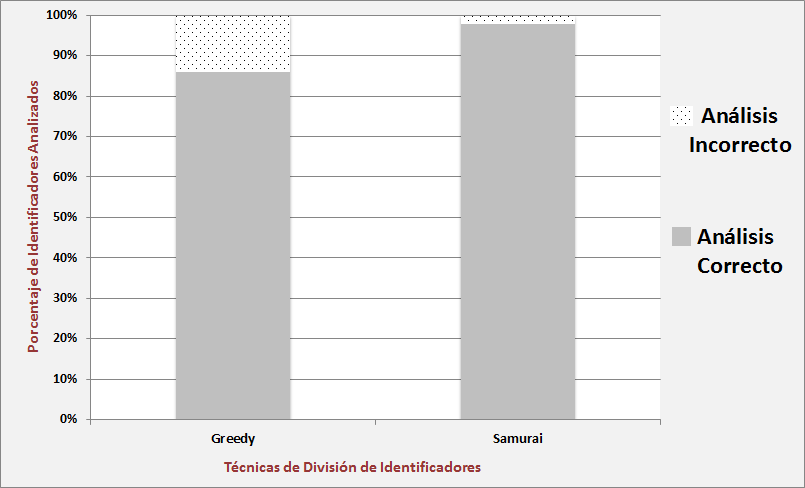
\includegraphics[scale= 0.66]{./cap5/barras_01.png}
}
\caption{Porcentajes de Ids divididos correctamente e incorrectamente}
\label{barras01}
\end{figure}

Una vez que IDA analizó alrededor de 400 ids en los tres casos de estudio presentados previamente, los resultados obtenidos de las divisiones se resumen en el gráfico de barras de la Figura \ref{barras01}. Como se puede observar en este gráfico, el eje vertical representa el porcentaje de ids analizados sobre la cantidad total. El color azul de cada barra indica que porcentaje sobre total de ids se separó correctamente, mientras que el rojo señala lo contrario. Por otro lado, el eje horizontal corresponde a cada una de las técnicas empleadas para dividir ids (Greedy, Samurai).
Claramente, el gráfico de la Figura \ref{barras01} muestra que entre las dos técnicas de división, Samurai contiene una tasa de fallo mucho menor que Greedy. Esto era previsible por que el algoritmo Greedy es bastante simple y divide sin tener en cuenta el contexto en el que esta situado el id, no ocurriendo lo mismo con Samurai, ya que emplea un análisis más complejo a la hora de realizar su tarea.

\begin{figure}[t!] %[h] para here [b] para bottom [t] para top
\centerline{%queda centrada mejor la imagen
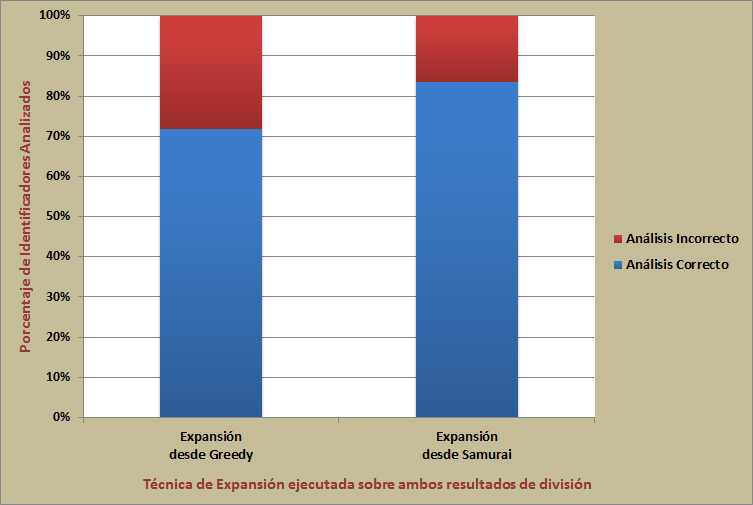
\includegraphics[scale= 0.64]{./cap5/barras_02.png}
}
\caption{Porcentajes de Ids expandidos correctamente e incorrectamente}
\label{barras02}
\end{figure}

Por otro lado, en la Figura \ref{barras02}, se aprecia una comparativa similar a la anterior, pero esta vez es entre las expansiones realizadas con la técnica de expansión básica, que recibe como entrada los dos grupos de resultados de las técnicas de división (Expansión desde Greedy y Samurai). Como se puede observar en la Figura \ref{barras02}, la expansiones de los ids que dividió Greedy tienen más casos incorrectos que las expansiones de los ids que dividió Samurai. Esto tiene sentido dado que mientras más acertada esté la división del id, mayor acierto tendrá la expansión. Si se compara las expansiones realizadas con las divisiones (Entre la Figura \ref{barras01} y \ref{barras02}), en el caso de las expansiones existe un aumento notable de casos incorrectos. Este comportamiento ocurre por que el algoritmo de expansión es básico y posee ciertos inconvenientes que fueron descriptos en el capítulo 3. Por último, las expansiones efectuadas luego de ser procesadas por el algoritmo Greedy son las que tienen mayor fallo, tomando en cuenta las dos figuras, esto ocurre debido a que se ejecutaron las dos técnicas más básicas y que más inconvenientes tienen (Greedy y Expansión Básica).

\enlargethispage{\baselineskip}
\enlargethispage{\baselineskip}%agrega linea al final de la hoja

Habiendo explicado los casos de estudio que muestran la utilidad de la herramienta IDA, en el próximo y último capítulo de este trabajo final, se describen las conclusiones obtenidas.